\todo{parler également de l'accélération}
Pour pouvoir proposer de nouvelles fonctionnalités de prévention, il faut optimiser le tableau de bord. Il faut créer des logos communs à tous pour avoir le même langage. 

\todo{ajout d'un tableau de bord connecté avec des capteurs et des alertes en temps réel.}
L'idée serait d'intégrer dans les motos une puce GPS qui serait capable d'avertir en cas de virage dangeureux. L'alerte (sonore via un intercom et voyant au tableau de bord) serait envoyée via le tableau de bord connecté si la vitesse est supérieure à 5 km/h à la vitesse limite autorisée. Généralement, les virages sont signalés par des panneaux et par une limitation de vitesse. Des chercheurs Alex Liniger et Simon Hecker ont développé un prototype , Aegis Rider AG\cite{vitesse_virage_mcnews} permettant de prendre la meilleure trajectoire. Cependant, ce dernier ne prend pas en compte les autres facteurs de la route (autres usagers, état de la chaussée, etc.). 

\begin{figure}[h]
    \centering
    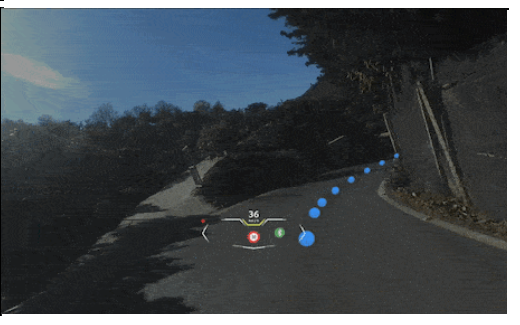
\includegraphics[width=0.7\textwidth]{coeur_memoire/images/aegis.png} 
    \caption{Prototype Aegis Rider AG pour la détection de virages dangereux.}
\end{figure}
Cette fonctionnalité est très interessante mais elle empêche une bonne visibilité de la surface de la route et elle peut fausser une prise de décision.
Comme illustré dans la Figure~\ref{fig:trajectoire_securite_difficulte}, le processus ne pourra pas adapter sur des virages dit "imparfaits".



\todo{mettre le diagramme}

\todo{Détailler le code}

\begin{tcolorbox}[title=Calcul de la courbure]
a + b = distance réelle parcourue en suivant la route \\
c = distance directe entre le début et la fin (comme si on traçait une corde)
\[
curvature = abs((a + b - c) / (a + b))
\]
\end{tcolorbox}


\todo{voir pour faire une petite ligne de code ?}
\lstinputlisting[language=Python]{coeur_memoire/programme1.py}

\todo{Mettre le budget pour développer la faisabilité}